\chapter{Analiza tematu}

W niniejszym opracowaniu zostaną przedstawione zagadnienia związane z~renderowaniem scen z wykorzystaniem metody ray marching oraz techniką tworzenia proceduralnie generowanego terenu.

Rozwiązania tego typu mogą być wykorzystywane w~obszarach związanych z~tworzeniem filmów, gier komputerowych, animacji itp. Ta metoda renderowania na dzień dzisiejszy nie jest jeszcze zbyt powszechna, a przynajmniej nie w takim stopniu jak metody oparte o rasteryzację trójkątów czy ray tracing.

Biorąc pod uwagę sposób działania technik renderowania opartych o wiązki światła, przedstawienie generowanego terenu wykorzystując siatkę trójkątów nie jest wydajnym rozwiązaniem. Wiąże się to z ilością obliczeń koniecznych do wykrycia kolizji z każdym trójkątem siatki dla każdej wiązki światła. Znacznie lepszym  i wydajniejszym rozwiązaniem jest przedstawienie terenu jako funkcji matematycznej.

Do kształtowania terenu w pierwszej kolejności zostanie wykorzystana funkcja zwracająca pseudolosową wartość dla danego dwuwymiarowego punktu\cite{bib:iqterrain}.
W tym celu można użyć z wielu różnych metod, przykładowo wykorzystując dwuwymiarową teksturę
lub funkcję matematyczną której wyniki przypominają losowe wartości. Aby uzyskać ciągłą funkcję, wartość każdego punktu jest interpolowana na podstawie czterech najbliższych punktów, których współrzędne są wartościami całkowitymi.

Aby uzyskać pożądany efekt zaimplementowana została interpolacja biliniowa opisana wzorem \ref{eq:interp-biliniowa}, dla wybranych punktów $a, b, c$ i $d$. Jako parametry tej funkcji $x$ i $y$ należą do przedziału $x, y \in [0, 1]$. Przykład tego rodzaju interpolacji przedstawia rysunek \ref{fig:lerp}.
\begin{equation}[H]
\label{eq:interp-biliniowa}
  \begin{split}
    f(x, y) & = a \\
       & + (b - a) x \\
       & + (c - a) y \\
       & + (a - b - c + d) x y
    \end{split}
\end{equation}

Można zauważyć, że efektem tej interpolacji są bardzo widoczne granice między grupami punktów, co przedstawia rysunek \ref{fig:linterp-edges}.

\begin{figure}
\centering
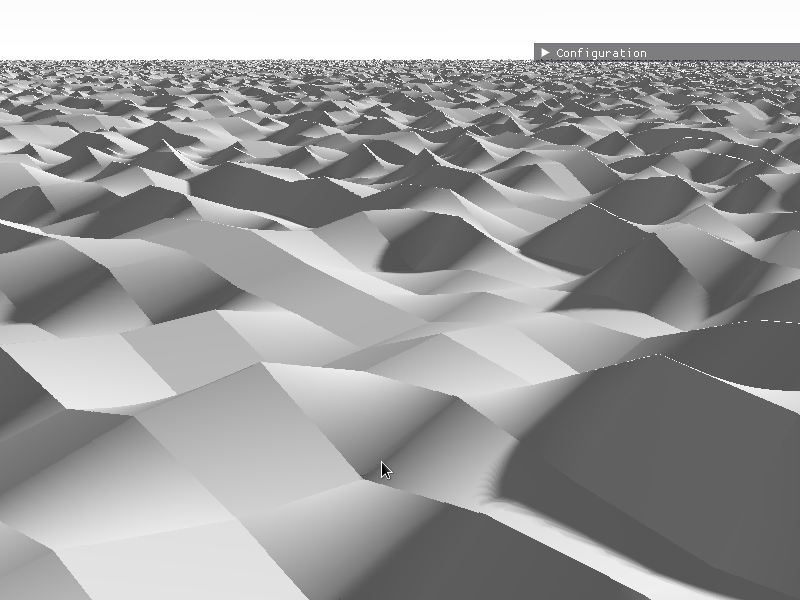
\includegraphics[width=0.65\textwidth]{./graf/ilin-edges.png}
\caption{Konfiguracja systemu budowy dla środowiska Visual Studio 16.}
\label{fig:linterp-edges}
\end{figure}


Rozwiązaniem tego problemu jest zastosowanie funkcji \ang{smoothstep} pozwalającej na uzyskanie wygładzonej interpolacji. W tym celu zmodyfikowano wzór \ref{eq:interp-biliniowa}, zastępując parametry $x$ i $y$ wykorzystując funkcję \ang{smoothstep} $n$-tego stopnia przedstawionej jako $S_n(p)$. Ostateczną postać funkcji przedstawia wzór \ref{eq:smooth-interp}. Obliczając gradient tej funkcji, można zauważyć, że wartości pochodnej dla każdego z czterech granicznych punktów jest równa $0$, dzięki czemu przejścia między grupami punktów nie są widoczne.

\begin{equation}
\label{eq:smooth-interp}
  \begin{split}
    f(x, y) & = a \\
       & + (b - a) S_n(x) \\
       & + (c - a) S_n(y) \\
       & + (a - b - c + d) S_n(x) S_n(y)
    \end{split}
\end{equation}

W programie wykorzystana została funkcja \ang{smoothstep} pierwszego stopnia, której postać jest widoczna na wzorze \ref{eq:smooth-interp-1}.

\begin{equation}
\label{eq:smooth-interp-1}
  \begin{split}
    S_1(x) = 3x^2 - 2x^3
  \end{split}
\end{equation}

Wynik zastosowania tego wzoru ukazuje rysunek \ref{fig:smooth-interp}.


\begin{figure}[H]
\centering
\subfloat[interpolacja biliniowa]{
  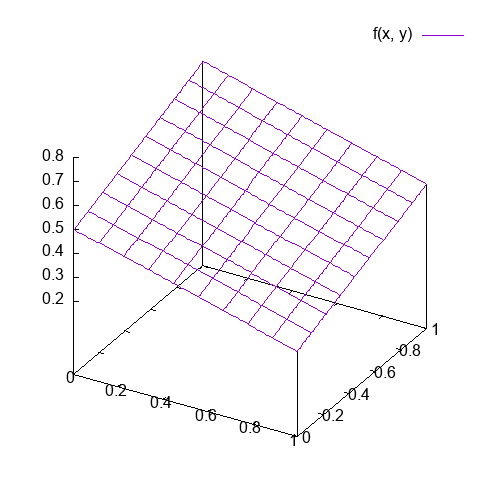
\includegraphics[width=0.5\textwidth]{./graf/plot/bilinear.png}
  \label{fig:lerp}
}
\subfloat[interpolacja wykorzystująca funkcję \ang{smoothstep} pierwszego stopnia]{
  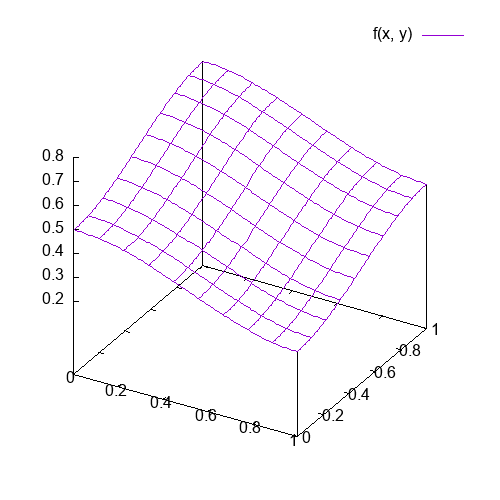
\includegraphics[width=0.5\textwidth]{./graf/plot/smooth.png}
  \label{fig:smooth-interp}
}
%% 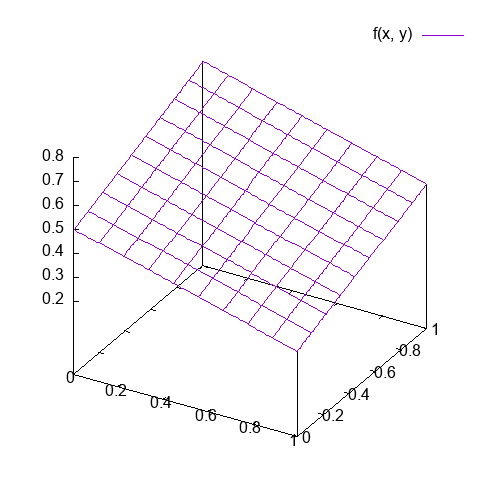
\includegraphics[width=0.65\textwidth]{./graf/plot/bilinear.png}
\caption{Porównanie wyników obu metod interpolacji między czterema punktami}
\label{fig:interpolacja}
\end{figure}

Uzyskany wynik jest zadowalający, jednak nadal nie przypomina naturalnego terenu. W celu poprawy jakości terenu można zastosować technikę o nazwie \ang{ułamkowe ruchy Browna} (\ang{fractional Brownian motion}, fBm)\cite{bib:bookofshaders}\cite{bib:Musgrave2003ProceduralFT}. Pożądany efekt można osiągnąć wykorzystując wzór \ref{eq:fbm}\cite{bib:iqfbm}, w którym $H$ jest wykładnikiem Hursta, a $N$ jest pożądaną ilością oktaw tej operacji.
\begin{equation}
\label{eq:fbm}
  \begin{split}
    fbm(p) = \sum^N_{k = 0} 2^{-Hk}f(2^kp)
  \end{split}
\end{equation}

W programie zastosowano wartość $H = 1$, gdyż wartość ta dała najbardziej realistyczne wyniki.
Zastosowanie stałej wartości $H$ daje bardziej uproszczony wzór, przedstawiony w postaci pseudokodu na rysunku \ref{fig:pseudokod:fbm}:

\begin{figure}[H]
\centering
\begin{lstlisting}[language=C]
float fbm(vec2 p) {
  float sum = 0.0;

  for (int i = 0; i < LAYERS; i++) {
    sum += pow(2, -i) * noise(pow(2, i) * p);
  }

  return sum;
}
\end{lstlisting}
\caption{Pseudokod funkcji \ang{fBm}.}
\label{fig:pseudokod:fbm}
\end{figure}

Kod z rysunku \ref{fig:pseudokod:fbm} został zmodyfikowany tak by zoptymalizować czas wykonania i uniknąć wykorzystania funkcji \ang{pow}\cite{bib:glslpow}. Wynikiem jest pseudokod z rysunku \ref{fig:pseudokod:fbm-opt}.

\begin{figure}[H]
\centering
%% \lstset{basicstyle=\ttfamily}
\begin{lstlisting}[language=C]
float fbm(vec2 p) {
  float sum = 0.0;
  float a = 1.0;

  for (int i = 0; i < LAYERS; i++) {
    sum += a * noise(p);
    p *= 2.0;
    a *= 0.5;
  }

  return sum;
}
\end{lstlisting}
\caption{Pseudokod funkcji \ang{fBm} po optymalizacji.}
\label{fig:pseudokod:fbm-opt}
\end{figure}

Po zastosowaniu powyższych działań uzyskano znacznie bardziej naturalny wynik. Dalsza analiza wygenerowanego terenu wykorzystując interpolację biliniową, przedstawiona na rysunku \ref{fig:fbm-bilin-align}, nasuwa wnioski, że wszystkie odkształcenia terenu biegną w jednej linii, co wpływa na naturalizm terenu. Aby uniknąć takiej sytuacji zmodyfikowano algorytm \ang{fBm} by oprócz skalowania współrzędnych punktu, zostały one także obrócone względem środka układu współrzędnych.

\begin{figure}
\centering
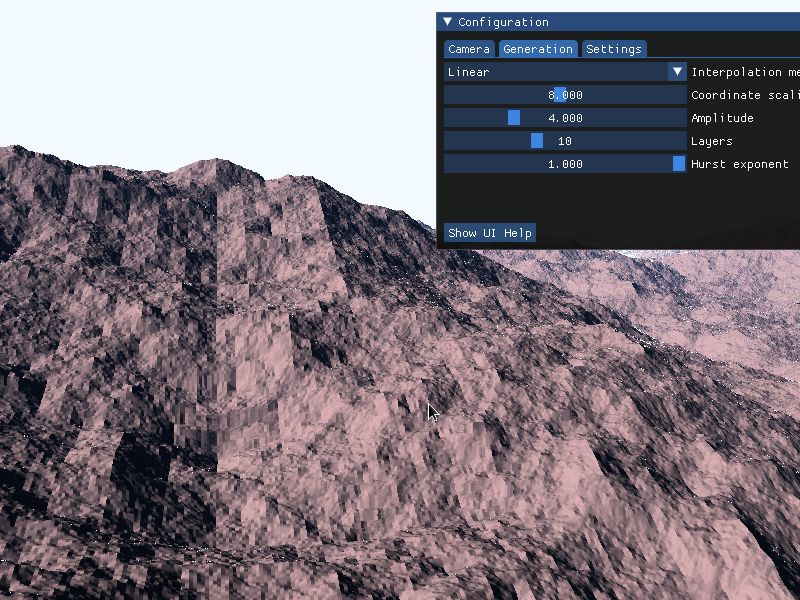
\includegraphics[width=1\textwidth]{./graf/fbm-bilin.png}
\caption{Wynik zastosowania \ang{fBm} dla 10 oktaw, z wykorzystaniem interpolacji biliniowej.}
\label{fig:fbm-bilin-align}
\end{figure}

%% \begin{itemize}
%% \item sformułowanie problemu
%% \item osadzenie tematu w kontekście aktualnego stanu wiedzy (\ang{state of the art}) o poruszanym problemie
%% \item  studia literaturowe \cite{bib:artykul,bib:ksiazka,bib:konferencja,bib:internet} -  opis znanych rozwiązań (także opisanych naukowo, jeżeli problem jest poruszany w publikacjach naukowych), algorytmów,
%% \end{itemize}


%% Wzory
%% \begin{align}
%% y = \frac{\partial x}{\partial t}
%% \end{align}
%% jak i pojedyncze symbole $x$ i $y$  składa się w trybie matematycznym.
